\part{Applications}

\chapter{Optimising for state fidelity}\label{chap:5_Applications_fidelity}

\section{Two-spin annealing}\label{sec:5.1_2spin_annealing}

One of the simplest example systems to illustrate the \acrref{COLD} method is that of a two-spin model and a simple annealing protocol:
\begin{equation}\label{eq:two_spin_hamiltonian}
H_0(\lambda) = -2J \sz_1 \sz_2 - h ( \sz_{1} + \sz_{2}) +  2h \lambda (\sx_{1} + \sx_{2}),
\end{equation}
where the Hamiltonian is parameterised by the set of coefficients $\{J, h, \lambda(t)\}$, with the $\lambda$ term encoding the time-dependence. For this example we use
\begin{equation}\label{eq:lambda_func1}
\lambda(t) = \sin^2\left(\frac{\pi}{2} \sin^2 \left( \frac{\pi t}{2 \tau} \right) \right),
\end{equation}
such that $\lambda(0) = 0$ and $\lambda(\tau) = 1$. In this way, the transverse field is tuned from $0$ to $2h$ as $t$ goes from $0$ to $\tau$.

\begin{equation}\label{eq:two_spin_alpha}
\alpha = - \frac{h^2}{4(h\lambda)^2 + h^2 + 4J^2}.
\end{equation}

\begin{equation}\label{eq:H_optimal_control}
H_\beta(\lambda) = H_0(\lambda) + \sum_{k=1}^{N_k} \beta^k \sin (\pi k \lambda) ( \sz_{1} + \sz_{2}),
\end{equation}

\begin{figure}[t]
    \centering
    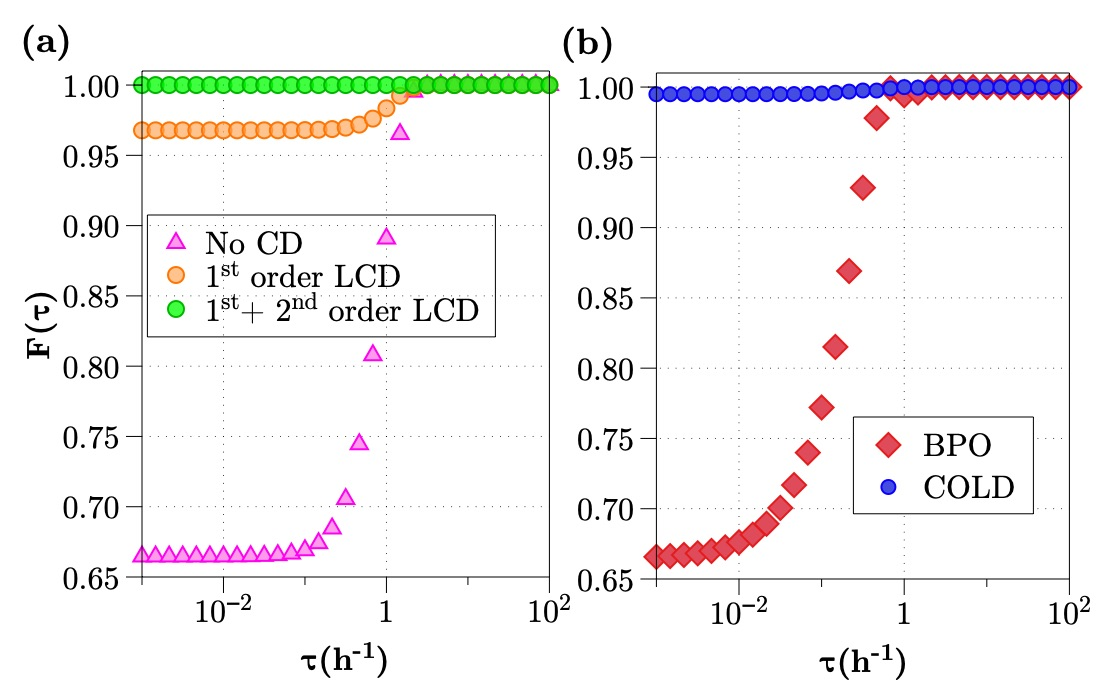
\includegraphics[width=0.9\linewidth]{images/twospins_fidelities.jpg} \caption[COLD applied to two-spin annealing]{}\label{fig:twospin_fidelities}
    \end{figure}

\section{Ising chain}\label{sec:5.2_Ising_chain}

\begin{equation}\label{eq:ising_chain_hamiltonian}
    H_0(\lambda) = - J \sum_{j}^{N-1} \sz_j \sz_{j+1} + Z_0\sum_j^N \sz_j + \lambda X_f \sum_j^N \sx_j,
\end{equation}

\begin{equation}
    \AGP{\lambda}^{(1)} = \alpha \sum_{j}^N\sy_j,
\end{equation}

\begin{equation}
    \alpha(\lambda) = \frac{1}{2} \frac{Z_0 X_f}{Z_0^2 + \lambda^2 X_f^2 + 2J^2}.
\end{equation}

\begin{equation}
    \AGP{\lambda}^{(2)} = \alpha \sum_{j} \sy_j + \gamma  \sum_{j} (\sx_j \sy_{j+1} + \sy_j \sx_{j+1}) +  \zeta \sum_{j} (\sz_j \sy_{j+1} + \sy_j \sz_{j+1}) ,
\end{equation}

\section{Transport in a synthetic lattice}

\begin{equation}\label{eq:lattice_hamiltonian}
    H_0(t) = - \sum_n J_n(t)(c_n^{\dag}c_{n+1} + H.c.) + \sum_n V_n(t) c_n^{\dag}c_n,
\end{equation}

\begin{align} \label{eq:J_lattice}
    J_n(t) &= J_0(1.1 - \lambda) \\ \label{eq:V_lattice}
    V_n(t) &= n V_0 2 (\lambda - 1/2),
\end{align}

\begin{equation}\label{eq:tunneling}
    J_n(t) \rightarrow J_{n, \mathrm{CD}}(t) e^{-i\phi_{n, \mathrm{CD}}(t)},
\end{equation}
where
\begin{align}\label{eq:J_cd}
    J_{n, \mathrm{CD}}(t) = \sqrt{J_n(t)^2 + (\alpha_n(t)/\tau)^2}, \\ \label{eq:phi_cd}
    \phi_{n, \mathrm{CD}}(t)  = \arctan\left(-\frac{J_n(t)\tau}{\alpha_n(t)}\right),
\end{align}

\section{Preparing GHZ states in a system of frustrated spins}\label{sec:6.4_ghz_states}

Multipartite entanglement is a powerful resource for quantum computing, quantum cryptography, quantum teleportation, and quantum metrology, offering unique capabilities for information processing, secure communication, high-precision measurements, and understanding the foundations of quantum mechanics. An example of such highly entangled states is the GHZ state on $N > 1$ spins:
\begin{equation}\label{eq:GHZ_state}
    \ket{\rm GHZ} = \frac{1}{\sqrt{2}} (\ket{0}^{\otimes N} + \ket{1}^{\otimes N}).
\end{equation}

GHZ states can be prepared via an annealing schedule on a system of frustrated spins. 

\begin{equation}\label{eq:ghz_hamiltonian}
    H_0(\lambda) = - J \Big( \sum_{j}^{N-1} \sz_j \sz_{j+1} + \sum_{j}^{N-2} \sz_j \sz_{j+2} \Big) - h(1 - \lambda) \Big( \sum_j^N (\sz_j + \sx_j) \Big).
\end{equation}

When $J$ is positive, the ground state of $H_0(1)$ is the GHZ state of Eq.~\ref{eq:GHZ_state}, whereas when it is negative 

While measuring the entanglement of a multipartite system is not quite as simple as in the bipartite case, there exists a notion of entanglement for a system of three spins: namely, the three-tangle, first introduced in Ref.~\cite{coffman_distributed_2000}, which not only captures 

Not the first time this is attempted with \acrref{CD}. \cite{sun_optimizing_2022}